\documentclass[11pt,a4paper,english,final]{article}
\usepackage[english]{babel} % Using babel for hyphenation
\usepackage{lmodern} % Changing the font
\usepackage[utf8]{inputenc}
\usepackage[T1]{fontenc}

%\usepackage[moderate]{savetrees} % [subtle/moderate/extreme] really compact writing
\usepackage{tcolorbox}
\tcbuselibrary{hooks}
\usepackage[parfill]{parskip} % Removes indents
\usepackage{amsmath} % Environment, symbols etc...
\usepackage{amssymb}
\usepackage{float} % Fixing figure locations
\usepackage{multirow} % For nice tables
%\usepackage{wasysym} % Astrological symbols
\usepackage{graphicx} % For pictures etc...
\usepackage{enumitem} % Points/lists
\usepackage{physics} % Typesetting of mathematical physics examples: 
                     % \bra{}, \ket{}, expval{}
\usepackage{url}

\definecolor{red}{RGB}{255,10,10}

% To include code(-snippets) with æøå
\usepackage{listings}
\lstset{
language=c++,
showspaces=false,
showstringspaces=false,
frame=l,
}

\tolerance = 5000 % Bedre tekst
\hbadness = \tolerance
\pretolerance = 2000

\numberwithin{equation}{section}

\newcommand{\conj}[1]{#1^*}
\newcommand{\ve}[1]{\mathbf{#1}} % Vektorer i bold
\let\oldhat\hat
\renewcommand{\hat}[1]{\oldhat{#1}}
\newcommand{\trans}[1]{#1^\top}
\newcommand{\herm}[1]{#1^\dagger}

\newcommand{\Real}{\mathbb{R}}
\newcommand{\bigO}[1]{\mathcal{O}\left( #1 \right)}

\newcommand{\di}{\mathrm{d}}

\newcounter{algcounter}
\renewcommand{\thealgcounter}{\Roman{algcounter}}

\newenvironment{algorithm}{%
\refstepcounter{algcounter}
\begin{tcolorbox}
\centerline{Algorithm \thealgcounter}\vspace{2mm}
}
{\end{tcolorbox}}

\newcommand{\figurewidth}{.85\textwidth}

\title{FYS3150 -- Computational Physics\\Project 3}
\author{Magnus Ulimoen}
\date{\today}

\begin{document}
\tcbset{before app=\parfillskip0pt}
\maketitle


\section{Introduction}
\label{sec:intro}

The goal of this project is to find the correlation energy between two 
electrons in the helium atom ground state. We do not have the analytical 
solution to this problem, so it is taken as an ansatz that the electrons 
can be superpositioned from hydrogen 1s-orbitals.

The program made to solve this problem 
can be found under the folder \url{Project3} in the github 
repository at \url{https://github.com/mulimoen/FYS3150CompPhy}, 
where all necessary information on how to run the program is included.

\section{Method}

\subsection{Wave function}

The 1s-orbital for hydrogen has a wave function given by
\begin{gather}
\psi(\ve{r}) = R_n(r)Y_l^m(\theta, \phi)
\end{gather}
For hydrogen in 1s, the wave function does not depend upon angles,
\begin{gather}
\psi(r) = C e^{-\alpha \frac{r}{a_0}}
\end{gather}
Where C is a normalisation constant and $\alpha$ is a parameter 
determing the strength of the potential. 
For our helium-atom this is chosen $\alpha = Z = 2$, corresponding to 
a charge of $2e$ for the nucleus of the helium atom. 
$r$ will be used in natural units, 
where $a_0 = 1$, and the normalisation constant is neglected.

The wave function for the electrons can not be found exact, but an 
ansatz can be taken, that the wavefunctions is simply two overlapping 
hydrogen 1s-orbitals.
\begin{gather}
\psi(r_1, r_2) = e^{-\alpha(r_1 + r_2)}
\end{gather}


\subsection{Interaction energy}

Since the electrons are not localized, but rather spread out over all the 
space, it is necessary to find the expectation value of the energy. 
Classically the energy between two charged objects are given by
\begin{gather}
V = k\frac{qQ}{\abs{\ve{r}_1 - \ve{r}_2}} = k\frac{qQ}{\abs{\ve{r}_{12}}}
\end{gather}
This suggest that the quantum mechanical interaction energy is the 
ensemble over all the space,
\begin{gather}
E_{\text{interaction}} \propto  
\expval{\frac{1}{\abs{\ve{r}_1 - \ve{r}_2}}}
\end{gather}
Which can be written out 
\begin{gather}
E_{int} \propto \int\!\! \int \conj{\psi} 
\frac{1}{\abs{\ve{r}_{12}}} \psi 
\,\, \di\ve{r}_1\di\ve{r}_2 = I
\label{eq:I}
\end{gather}
An analytical solution of this is
\begin{gather}
I = \frac{5\pi^2}{16}
\end{gather}



\subsubsection{Cartesian coordinates}

The integral \eqref{eq:I} takes the following form in cartesian 
coordinates,
\begin{gather} I = 
\int\!\!\int\!\!\int\!\!\int\!\!\int\!\!\int
\frac{e^{-2\alpha\left(\abs{\ve{r}_1} + \abs{\ve{r}_2 }\right)}
}{\abs{\ve{r}_{12}}}
\di x_1\di y_1\di z_1\di x_2\di y_2\di z_2
\label{eq:IC}
\end{gather}
with all the limits from $-\infty$ to $\infty$. 


\subsubsection{Polar coordinates}
Since the integral constains a large amount of radial elements,
a change to polar coordinates leads to 
better algorithms and solutions.

In order to change into polar coordinates we need to have the Jacobi 
determinant, also called volume 
element $\di V$. In polart coordinates this takes the form
\begin{gather}
\di V = r^2\sin\theta \di r\di\theta\di\phi
\end{gather}
The term $\abs{\ve{r}_1 - \ve{r}_2}$ is expressed in these coordinates
\begin{gather}
\abs{\ve{r}_1 - \ve{r}_2} = \abs{r_1 \ve{e}_{r_1} - r_2\ve{e}_{r_2}}
 = \sqrt{(r_1 \ve{e}_{r_1} -  r_2\ve{e}_{r_2})\cdot 
 (r_1 \ve{e}_{r_1} - r_2\ve{e}_{r_2})}\\
 = \sqrt{r_1^2\ve{e}_{r_1}^2 + r_2^2\ve{e}_{r_2}^2  
 - 2r_1r_2 \ve{e}_{r_1}\cdot \ve{e}_{r_2}}
\end{gather}
The inner product of $\ve{e}_{r_i}$ with itself is one. It is necessary 
to find the dot product $\ve{e}_{r_1}\cdot \ve{e}_{r_2}$ which is the 
angle between the two unit vects, $\cos\beta$.
Writing out the radial unit vector in 
polar coordinates,
\begin{gather}
\ve{e}_r = \cos\phi\sin\theta \ve{i} + \sin\phi\sin\theta\ve{j} 
+ \cos\theta\ve{k}
\end{gather}
The inner product of the two radial unit vectors are 
\begin{gather}
\cos\beta = \cos(\theta_1)\cos(\theta_2)
+ \sin(\theta_1)\sin(\theta_2)\cos(\phi_1 - \phi_2)
\label{eq:cosbeta}
\end{gather}
And the integral \eqref{eq:I} takes the form
\begin{gather} I = 
\int\limits_0^{2\pi}\!\int\limits_0^{2\pi}\!
\int\limits_0^\pi\!\int\limits_0^\pi\!
\int\limits_0^\infty\!\int\limits_0^\infty 
\frac{r_1^2r_2^2 e^{-2\alpha(r_1 + r_2)} \sin(\theta_1)\sin(\theta_2)
}{\sqrt{ r_1^2 + r_2^2 - 2r_1r_2\cos\beta }}
\di r_1\di r_2\di\theta_1 \di\theta_2 \di\phi_1 \di\phi_2
\label{eq:IR}
\end{gather}

\section{Numerical approximations}

To solve this integral some precautions must be taken.
A straight forward method requires all of the space to be integrated,
which is unfeasable numerically. 
The function should only be integrated where it is interesting, which 
is close to origo to due the exponential part. A suitable limit 
is selected based on where the wave function is approximately zero.

Another problem is the singularity that arises when $\ve{r}_{12}$ is zero. 
This is solved by not letting this part contribute if this occurs, as 
this volume is of very limited size and should not contribute much 
to the value of the integral.

If weights and mesh points are used we obtain a large amount of
intertwined 
variables that needs to be permuted. This gives a complexity of 
$N^6$ calculations for the integral.
This requires effective weights and mesh points to solve, and Gauss 
Quadrature is used. Another method is Monte Carlo integration which 
does not depend on weights.

\subsection{Gauss Quadrature}

The Gauss Quadrature uses orthogonal polynomials to capture the 
function in its space and gives weights and meshpoints which is 
summed over. The two methods used are based on Legendre polynomials 
and Laguerre polynomials.

\subsubsection{Legendre}

The Legendre quadrature uses the weight function 
\begin{gather}
I = \int_a^b f(y) dy = \int_{-1}^1 W(x) f(x) dx 
\approx \sum_i w_i f(x_i)
\end{gather}
and meshpoints as the zeros of the Legendre polynomial. 
The legendre polynomials are defined for integrals with limits $[-1,1]$.
A linear mapping is used, which maps the limits to $[0,\text{limit}]$.

\subsubsection{Laguerre}

This Laguerre quadrature uses the weight function
\begin{gather}
I = \int f(y) dy = \int_0^\infty \frac{W(x)}{x^{\tilde{\alpha}} e^{-x}} f(x) dx
\approx \sum_i w_i f(x_i)
\end{gather}
In \eqref{eq:IR} we have a factor which strongly resembles the dividing 
factor of the above equation. If the choice $x_i = 2\alpha r_i$ is made 
and $\tilde{\alpha} = 2$,
the integral simplifies to 
\begin{gather}
I = \int\!\cdots\!\int \frac{r_1^2e^{-x_1}}{x_1^2e^{-x_1}}
\frac{r_2^2e^{-x_2}}{x_2^2e^{-x_2}} 
\frac{W(x_1)W(x_2)}{\abs{\ve{r}_{12}}} \cdots
\di r_1 \di r_2 \cdots
\end{gather}
Changing the variables and considering 
\begin{gather}
\abs{\ve{r}_{12}} = \frac{\abs{\ve{x}_{12}}}{2\alpha}
\end{gather}
the integral simplifies further,
\begin{gather}
\nonumber I = 
\frac{1}{(2\alpha)^5}\sum_{i, j, \cdots} 
\frac{w(x_{1,i})w(x_{2,j})}{\abs{\ve{x}_{12,ij}}} 
\sin\theta_{1,k} \sin\theta_{2,l} w(\theta_{1,k}) w(\theta_{2,l})
w(\phi_{1,m}) w(\phi_{2,n})
\end{gather}
With the sum taken over all the permutations of $i,j, \cdots$.



\subsection{Monte Carlo}

The Monte Carlo approach is picking out the numbers randomly from a range
and then 
calculating the average value of the function with these numbers.
As the number of guesses 
increases the integral should approach the true value. Since the Monte 
Carlo is random there is also a need to get the variance in order 
to get an error estimate. The variance is calculated through
\begin{gather}
\mathrm{Var}(X) = \expval{x^2} - \expval{x}^2
\end{gather}
To compare over several values of $N$ the standard deviation is used,
\begin{gather}
\sigma = \sqrt{\frac{\mathrm{Var}(X)}{N}}
\end{gather}
The random number generators should produce a uniform distribution
in the range $[0,1]$. Since the integral selected here does not have these 
limits a change of variables is needed. This could either be used in a 
straight forward method of linear mapping, 
or some more clever approches could be employed.


\subsubsection{Brute force}

The integral \eqref{eq:IC} can be solved by setting the artifical limits 
$[-\mathrm{limit}, \mathrm{limit}]$ and doing a linear mapping to these limits.
This causes the volume $\di x_1 \di y_1 \cdots$ to depend on the 
limit chosen as $(2\text{ limit})^6$, which can be imaginged as the size
of the ''box'' which is integrated over. A pseudo-code for this is
\begin{lstlisting}
gen = random_number(-limit, limit)

repeat N times {
x1 = gen()
x2 = gen()
y1 = gen()
 ...

r1 = x1*x1 + y1*y1 + z1*z1
r2 = x2*x2 + ...

r12 = sqrt((x1-x2)*(x1-x2) + ...)
f = exp(-2*alpha*(r1 + r2)/sqrt(r12)
sum = sum + f
square_sum = square_sum + f*f
} // end repeat

norm_factor = (2*limit)^6

sum = sum*norm_factor
square_sum = square_sum*norm_factor^2

mean = sum/N*norm_factor
Var = square_sum/N  - mean*mean
std_dev = sqrt(Var/N)
\end{lstlisting}

Another way to implement the brute force Monte Carlo is using the 
polar coordinates. The sphere is then mapped to a cube with the 
linear mapping 
$\theta = [0, \pi]$, $\phi = [0, 2\pi]$, $r = [0,\mathrm{limit}]$. 
The volume of this box is now $\pi^2(2\pi)^2(2\mathrm{limit})^2$.

\subsubsection{Importance sampling}

The brute force method does not follow the rapidly varying nature of 
the function which is integrated. The sampling of the random variables 
should therefore be adapted to take this into account. Both the 
angular part and the radial part is considered.

Simplifying the spherical part is done by considering the factor 
$\sin\theta \di\theta$. Comparing this with $\cos \theta$,
\begin{gather}
\frac{d\cos \theta}{d\theta} = \sin\theta\\
d\cos\theta = \sin \theta d\theta
\end{gather}
If now replacing $\cos \theta$ with $x$, and let this variable be selected 
by the uniform distribution in the range $[-1,1]$ we can rewrite 
\eqref{eq:cosbeta} to use this choice of variable,
\begin{gather}
\cos\beta = x_1 x_2 + \sqrt{1-x_1^2}\sqrt{1-x_2^2}\cos(\phi_1-\phi_2)
\end{gather}
Which also give the normalisation factor $2$ to the integral.

For the radial part an exponential distribution is chosen.
This distribution transforms the integral to
\begin{gather}
\int_0^\infty p(y)f(y) dy = \int_0^1 \frac{f(y(x))}{e^{-y}} dx
\end{gather}
With $y$ given by the inverse of the distribution

The integral in \eqref{eq:IR} has the form
\begin{gather}
\int_0^\infty \!\! dr \,\, r^2e^{-2\alpha r} f(r)\cdots
\end{gather}
Making the change of variables
\begin{gather}
y = 2\alpha r = \frac{r}{\lambda}\\
y = -\lambda\ln(1-x)
\end{gather}
Where x is the random number generated by a RNG. The integral needs to 
be transformed to be usable with these new numbers,
\begin{gather}
I = \lambda^2 2^2
\int\limits_0^{2\pi} \! \int\limits_0^{2\pi} \!
\int\limits_0^1 \!\!\int\limits_0^1 \!\!\int\limits_0^1\!\!
\int\limits_0^1 
\frac{y_1^2y_2^2 }{\abs{\ve{y}_{12}}}
\di x_1 \di x_2 \di x_3 \di x_4 \di \phi_1 \di \phi_2
\end{gather}
Or as a sum 
\begin{gather}
I = \frac{(2\cdot 2\pi \cdot \lambda)^2}{N}\sum 
\frac{y_1^2y_2^2 }{\abs{y_1^2+y_2^2 -2y_1y_2\cos\beta}}
\end{gather}




\section{Implementation}

The programming language used is C++, and the code is available in the 
github repository listed in section \ref{sec:intro} which also 
contains a README on how to use this program. The program source 
code is under \url{src}. A short description of the algorithms used 
follows in this section.


\subsection{Gauss Quadrature}

\subsubsection{Pure Legendre}

Mapping of the integral is done by a call to a function which gets the 
weights and mesh points by finding the roots of the appropriate 
polynomail. This is integrated by looping over the six 
variables which all uses the same weights and meshpoints, and summing 
the appropriate sum.

\subsubsection{Laguerre and Legendre}

The weights and meshpoints are found by 
a call to the appropriate function. The angles $\theta$ and $\phi$
are still mapped using 
the Legendre method. The summing of the appropriate sum gives the 
integral.


\subsection{Monte Carlo}

In order to extract the random numbers a RNG is used. The function used 
is the Mersenne Twister from the standard library, defined in the 
<random> header. To avoid initializing the same seed only one generator 
is used in this program. This might cause a loss of performance 
if operating with several threads, but this is assumed to be 
negligible.

These algorithms are coded so that they can be run in parallel using 
OpenMP. This should give a speedup of the program execution.


\subsubsection{Brute force}

The RNG is bound with the real uniform distribution defined in the 
standard library. For the cartesian coordinates the mapping 
$[-\mathrm{limit}, \mathrm{limit}]$ is used. In polar coordinates
three different distributions are made to get the appropriate 
limits.



\subsubsection{Importance sampling}

The RNG is bound with the exponential distribution defined in the 
standard library. A lambda function is used so a call to this function 
will combine four random numbers into $\cos\beta$. The sum is then 
calculated and the mean and standard deviation is calculated.

\section{Results}

The analytical result is known to be
\begin{gather}
I = \frac{5\pi^2}{16} = 0.192765711
\end{gather}


\subsection{Gauss Quadrature}


The results for the Gauss Legendre approach is in table \ref{table:GLE}.
The Gauss Laguerre approach are listed in table \ref{table:GLA}. Both of 
these are plotted against the relative error in figure \ref{fig:GQ}.


\begin{table}
\centering
\caption{Results for the Gauss-Legendre approach} \vspace{2mm}
\begin{tabular}{|c|c|c|c|} \hline
N & Result & Relative error & Limit \\ \hline
10 & 0.071979677 & 0.627 & 3\\
10 & 0.011164658 & 0.942 & 5\\
10 & 0.000011218 & 1.000 & 10\\ \hline
15 & 0.239088291 & 0.240 & 3\\
15 & 0.315862997 & 0.639 & 5\\
15 & 0.135901531 & 0.295 & 10\\ \hline
20 & 0.156139391 & 0.190 & 3\\
20 & 0.096788762 & 0.498 & 5\\
20 & 0.009799632 & 0.949 & 10\\ \hline
25 & 0.195816565 & 0.016 & 3\\
25 & 0.240135013 & 0.246 & 5\\
25 & 0.307075670 & 0.593 & 10\\ \hline
30 & 0.177282956 & 0.080 & 3\\
30 & 0.146370604 & 0.024 & 5\\
30 & 0.051521493 & 0.733 & 10\\ \hline
35 & 0.189923139 & 0.014 & 3\\
35 & 0.204704919 & 0.062 & 5\\
35 & 0.298264908 & 0.547 & 10
\\ \hline
\end{tabular}
\label{table:GLE}
\end{table}

\begin{table}
\centering
\caption{Results for the Gauss-Laguerre approach} \vspace{2mm}
\begin{tabular}{|c|c|c|} \hline
N & Result & Relative error\\ \hline
10 & 0.186457345 & 0.0327 \\
15 & 0.189758982 & 0.0156 \\
20 & 0.191081780 & 0.0087 \\
25 & 0.191740740 & 0.0053 \\
30 & 0.192113712 & 0.0033 \\
35 & 0.192343301 & 0.0021
\\ \hline
\end{tabular}
\label{table:GLA}
\end{table}


\begin{figure}
\centering
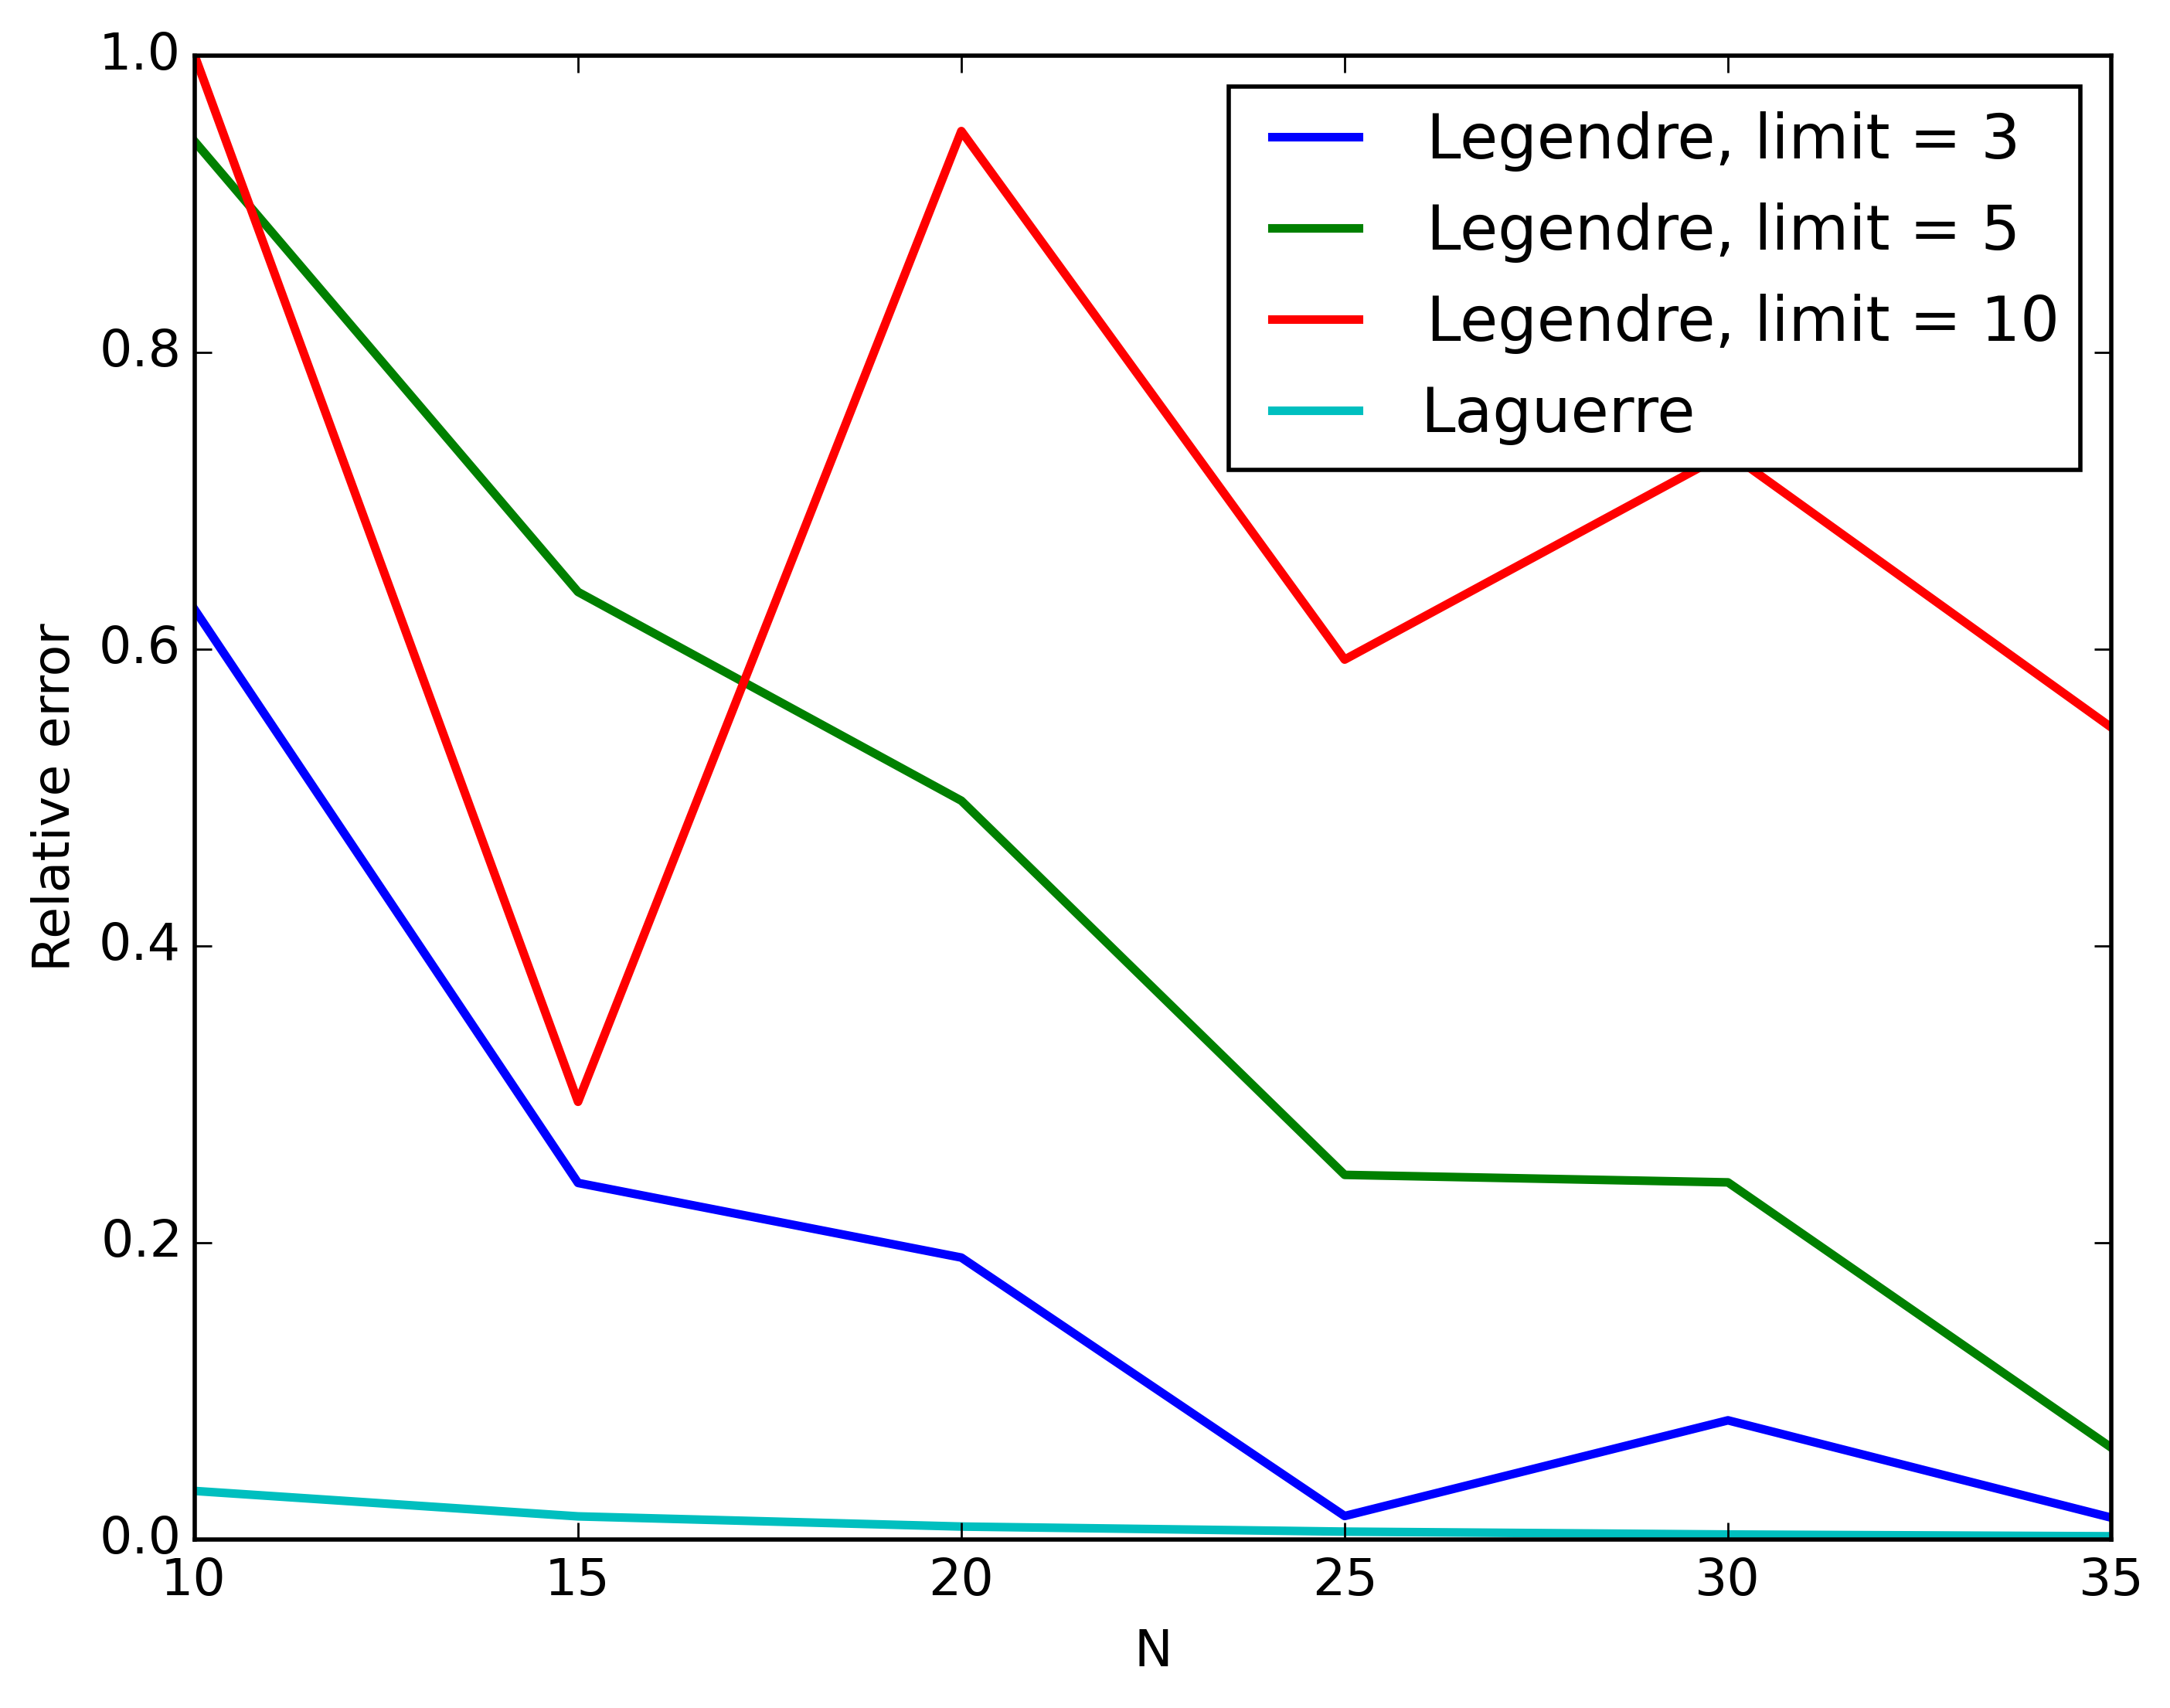
\includegraphics[width=\figurewidth]{analyse/GQ_error.png}
\caption{Plot of the relative error for the Gauss Legendre and Gauss
Laguerre approach
with different values of N and the limit}
\label{fig:GQ}
\end{figure}


\subsection{Monte Carlo}

A table over the result of typical Monte Carlo runnings is included 
in table \ref{table:MCC}, table \ref{table:MCP} and 
table \ref{table:MCI}. A figure 
which shows the estimated value of the integral for the different
algorithms are 
included in figure \ref{fig:MC}.

The implementation of OpenMP leads to a decrease of time for the execution.
It is however not optimal, as the speedup is 1.5 when using 4 threads,
compared to an optimal speedup of 4.



\begin{table}
\centering
\caption{Results for Monte Carlo in cartesian coordinates} \vspace{2mm}
\begin{tabular}{|c|c|c|} \hline
N & Result & Standard deviation\\ \hline
10 & 0.000000008 & 0.000000007\\
100 & 0.001133467 & 0.001125540\\
1000 & 0.024285372 & 0.023123862\\
10000 & 0.014531879 & 0.005365095\\
100000 & 0.194244256 & 0.086522718\\
1000000 & 0.117016553 & 0.027317216\\
10000000 & 0.206257811 & 0.040739848\\
100000000 & 0.185448419 & 0.012420672\\ \hline
\end{tabular}
\label{table:MCC}
\end{table}

\begin{table}
\centering
\caption{Results for Monte Carlo in polar coordinates} \vspace{2mm}
\begin{tabular}{|c|c|c|} \hline
N & Result & Standard deviation\\ \hline
10 & 0.000376852 & 0.000145215\\
100 & 0.231511633 & 0.126265106\\
1000 & 0.157525515 & 0.027329668\\
10000 & 0.212161377 & 0.016812296\\
100000 & 0.197445741 & 0.004107642\\
1000000 & 0.206297434 & 0.007374732\\
10000000 & 0.198070682 & 0.000595095\\
100000000 & 0.200285570 & 0.000732391\\ \hline
\end{tabular}
\label{table:MCP}
\end{table}

\begin{table}
\centering
\caption{Results for Monte Carlo importance} \vspace{2mm}
\begin{tabular}{|c|c|c|} \hline
N & Result & Standard deviation\\ \hline
10 & 0.240731444 & 0.133228794\\
100 & 0.412266740 & 0.177025271\\
1000 & 0.169150179 & 0.025264961\\
10000 & 0.190142914 & 0.006359748\\
100000 & 0.193869185 & 0.002517490\\
1000000 & 0.193403734 & 0.000843820\\
10000000 & 0.195505813 & 0.000325820\\
100000000 & 0.195270296 & 0.000270642\\ \hline
\end{tabular}
\label{table:MCI}
\end{table}


\begin{figure}
\centering
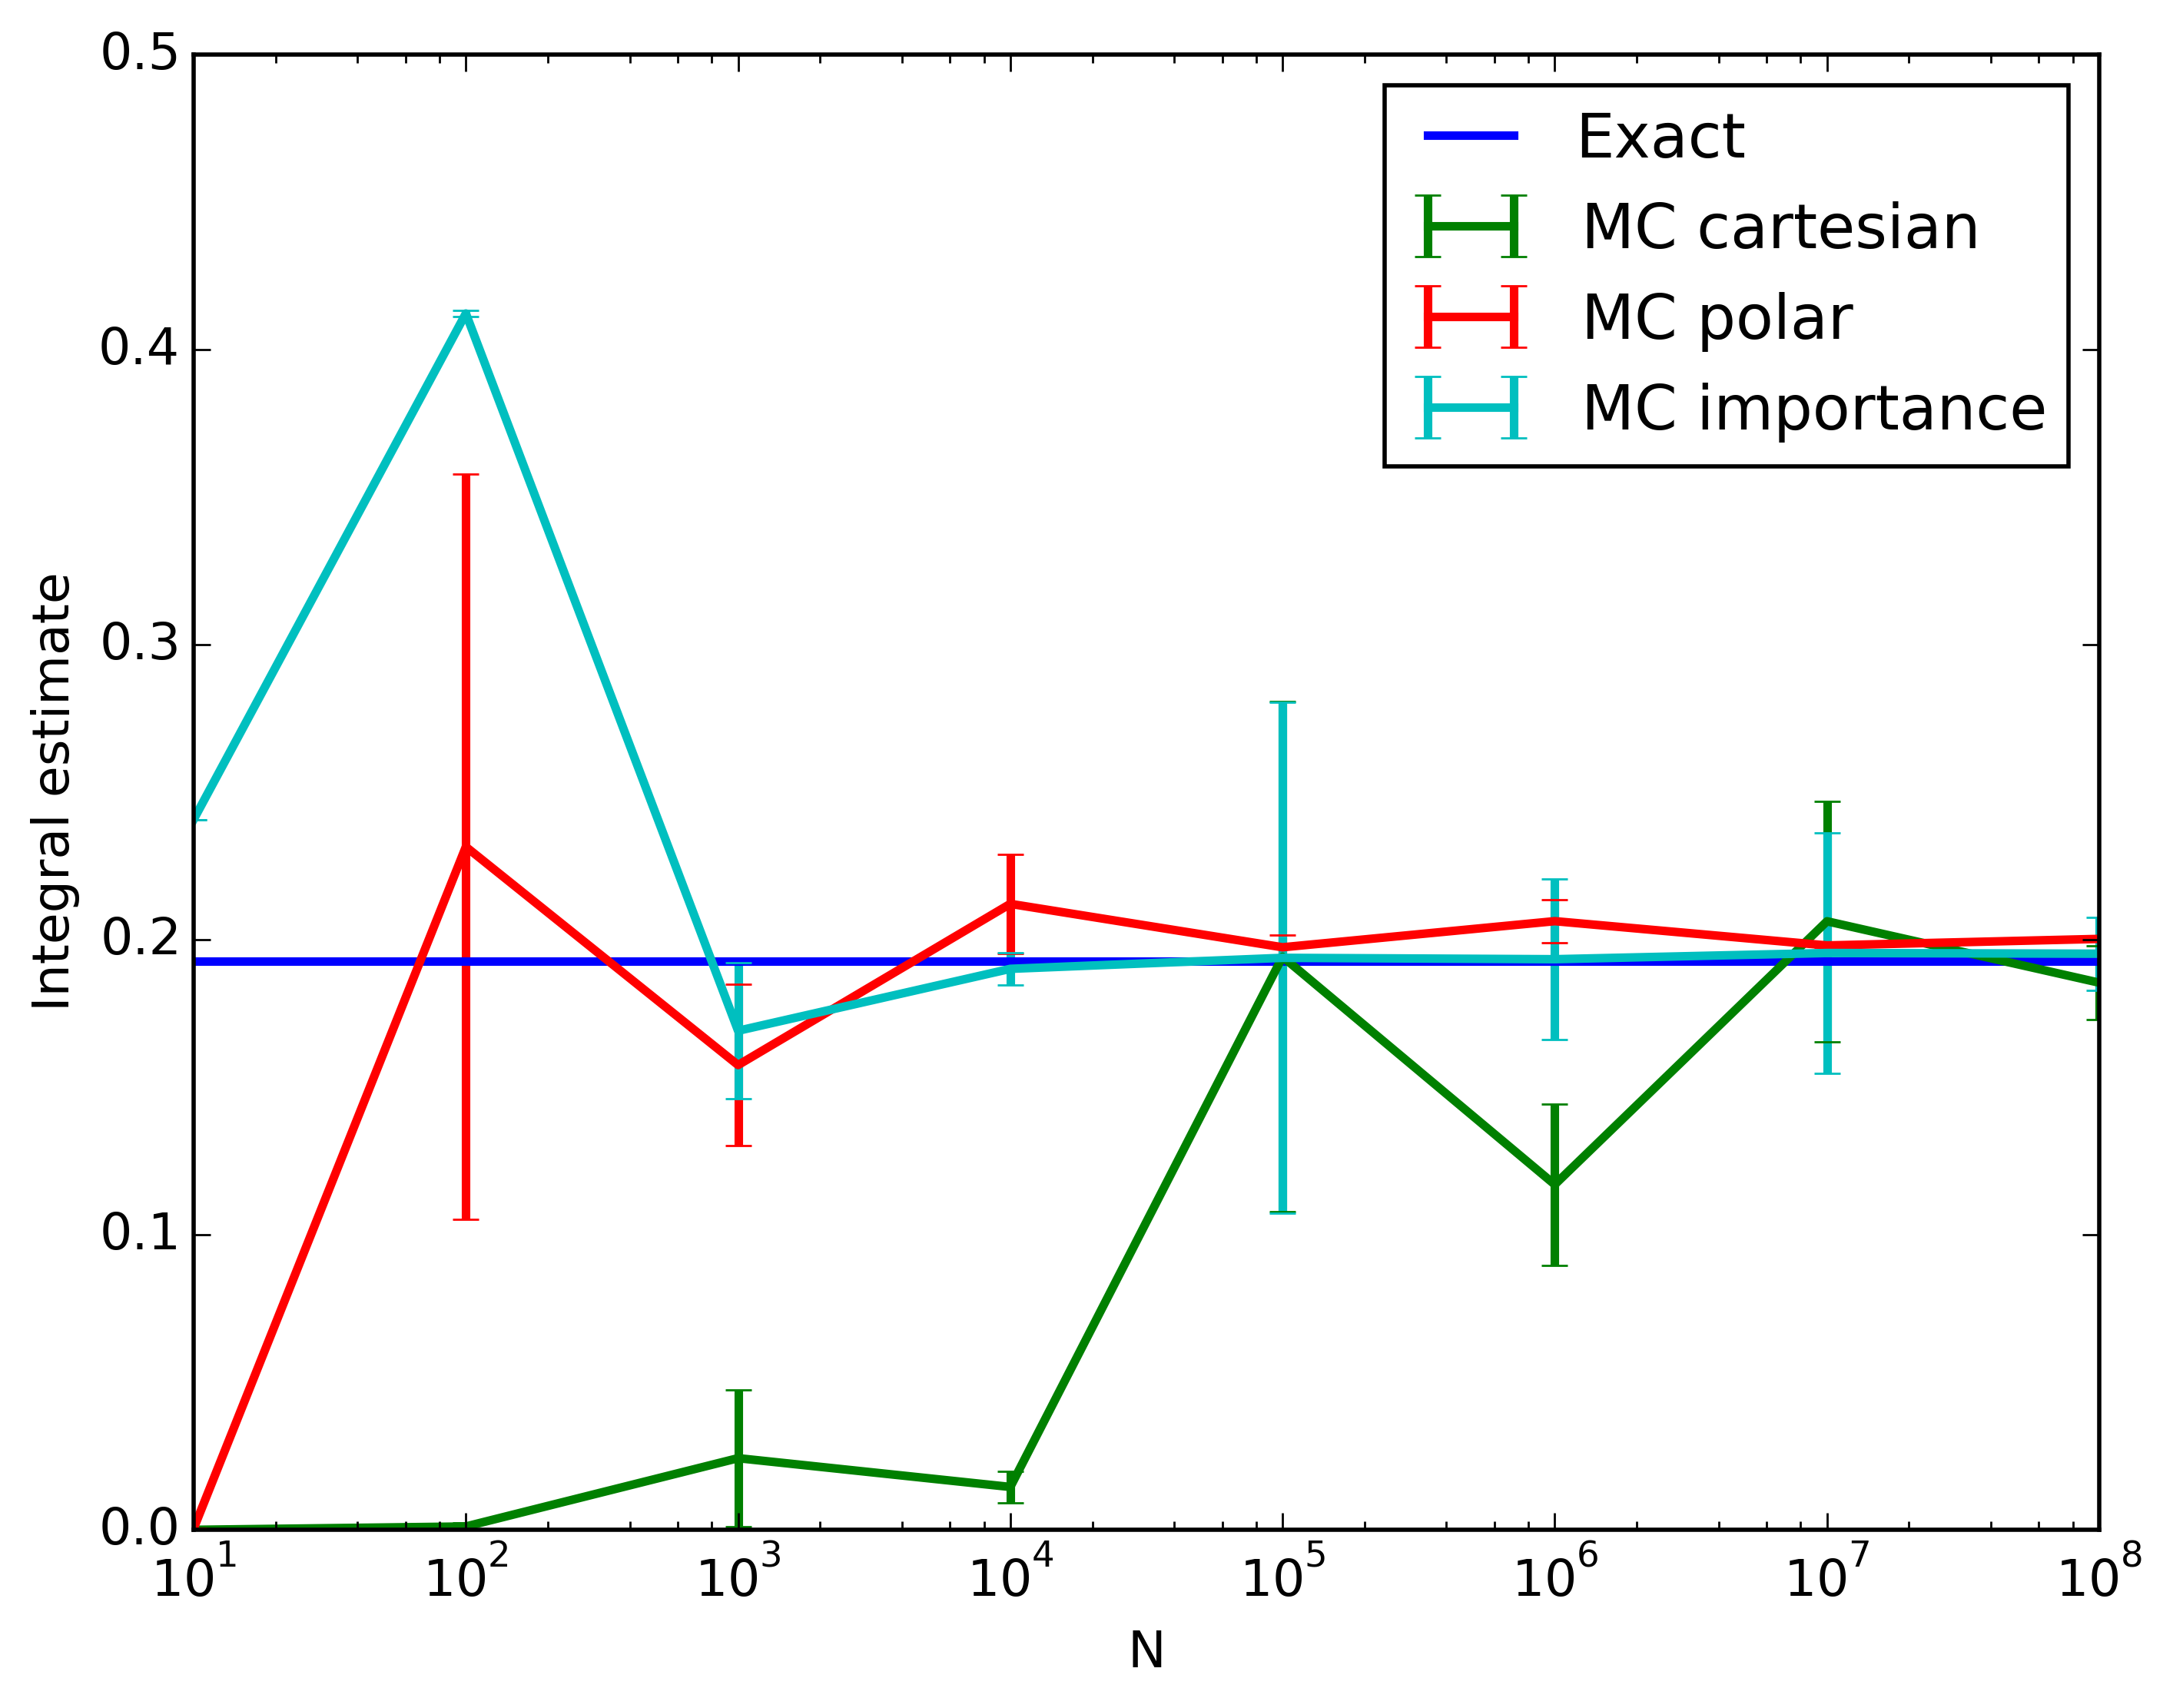
\includegraphics[width=\figurewidth]{analyse/MC_error.png}
\caption{Values of the integral along with the standard deviation as 
error bars for 
different values of N for the three methods employed.}
\label{fig:MC}
\end{figure}

\begin{table}
\centering
\caption{Program time in seconds for the parallelisation in MC methods, 
run with N = 10000000, * marks number of virtual cores on the tested
computer}
\vspace{2mm}
\begin{tabular}{|c|c|c|c|} \hline 
Number of threads & Time MCC & Time MCP & Time MCI\\ \hline
1 & 1.50 & 2.75 & 2.17\\
2 & 1.26 & 2.12 & 1.85\\
4* & 0.97 & 1.75 & 1.44\\
8 & 0.99 & 1.77 & 1.48\\ \hline
\end{tabular}
\label{table:MCtime}
\end{table}

\section{Discussion}

The algorithms used here do all tend to converge to the analytical 
solubtion if 
suitable parameters are used. But since the rate of convergence for 
some of these are too low, they will never converge to a meaningful 
value before roundoff errors and computational complexity overtakes it.

The approach based on Gauss-Legendre is unstable and good parameters 
must be selected to ensure that it comes close enought to the solution.
The Laguerre approach gives far more satisfiable approximations, and 
quicly reaches three digit precision.


As the Monte Carlo methods rely on randomness the estimate can be quite 
off the true analytical solution. With higher values of $N$ all the three 
algorithms converges to the true solution, but the rate of convergence
is differing. 
The brute force method based on cartesian coordinates do not converge 
to more than a digit for $N = 10^8$ as the sampling does not capture 
the function. 
Changing to polar coordinates gives a better way to sample the space, 
and leads to better results. The 
importance sampling gives results which are better than both of these 
methods.

The standard deviation as a mesure of the error is according to the 
plot \ref{fig:MC} sometimes connected to a high degree of randomness. 
For some of the data points the error estimate is far lower than 
the real value. A better approach to estimate the error should be 
sought after.

The time to run these programs shows that MCC is the fastest for a given N.
This is explained by the operations used. MCC only uses three 
expensive\footnote{ Exponentions, trigonometric and square root}
functions per calculation,
MCP uses 9 expensive functions per calculation while MCI uses 4. This
should be weighted against the accuracy gained from the different methods,
which clearly favours MCI. 

The speedup when using OpenMP is not optimal. Although a small speedup is
achieved, the optimalisation does not use all the virtual cores 
optimally. One reason for this could be the random number generator. 
Since there is only one RNG for all threads, here could be some idling 
of the threads when waiting for this to be available. Future 
implementations should create a thread-local RNG to avoid this idling.






\end{document}
